\subsection{Dominant topologies}

The statistics given in Figure~\ref{fig:sbndStats} indicate that the dominant interactions observable in SBND will be CC0$\pi$ and the CC1$\pi ^{\pm}$, example Feynman diagrams of these processes are given in Figure~\ref{fig:feyn}. 

    \begin{figure}[h!]
        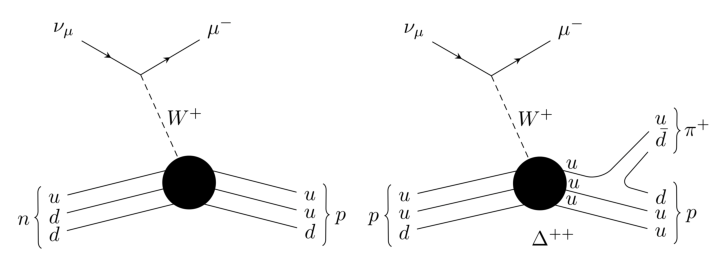
\includegraphics[width=\textwidth]{images/feynmans.pdf}
        \caption{On the left-hand side is a Feynman diagram of the CC0$\pi$ interaction with 1 proton in the final state. During this process, the incoming neutrino interacts with a neutron and produces a muon and a single proton as the observable final state particles. On the right is the postive version of the CC1$\pi ^{\pm}$ interaction, in which a neutrino interacts with a proton emitting a $\pi ^{+}$ alongside the final state muon and proton. Here, the invariant mass of the entire hadronic system must be accounted for when reconstructing the neutrino energy.}
        \label{fig:feyn}
    \end{figure}
    
    The energy of the incoming neutrino must be reconstructed from the other particles involved in the interaction. When dealing simply with a 2-body hadronic process, such as the one shown in the left hand side of Figure~\ref{fig:feyn}, it is acceptible to use the quasi-elastic estimation~(\ref{eq:Ereco}) \cite{teppei} to calculate the reconstructed energy, $\bar{E}_{\nu}$. Where $E_{\mu}, m_{\mu}$ and $\underline{k}'_{\mu}$ are the energy, mass and 3-momentum of the final state muon, $M_{N}$ is the mass of a target nucleon and $\theta$ is the opening angle between the outgoing muon and proton.  


    \begin{equation}\label{eq:Ereco}
        \bar{E}_{\nu} = \frac{ E_{\mu} - m^{2}_{\mu} / (2M_{N}) }{ 1 - ( E_{\mu} - |\underline{k}'_{\mu}| cos \theta ) / M_{N} }
    \end{equation}

Alternatively, if the interaction involves the existence of more particles in the final state, such as multiple protons or pions escaping the nucleus, one must account for the energy given to all of the hadronic final state particles in the energy reconstruction. 


    % Plan
    \begin{itemize}
        \item Importance of making sure the analysis framework is good enough
        \item What we will see
        \item How impurities affect signal
        \item Potential backgrounds 
        \item Importance of characterising the backgrounds
    \end{itemize}

\subsection{Preliminary categorisation exercise}
    
    % Plan
    \begin{itemize}
        \item Preliminary tests to determine what the signal and background will look like
        \item MC produced using SBND flux shape and magnitude 
        \item Smearing the MC to account for potential detector effects
        \item Energy resolution of SBND and inclusion in the smearing
        \item Impurity due to some pion characteristics
        \item Improvements to this which would be more realistic
        \item This will be better implemented in LArSoft using full detector simulation
        \item Categorizing the signal and could-be backgrounds
        \item Efficiency and purity definitions for the detector
        \item Identifying what will be the interesting channels in SBND
    \end{itemize}


\clearpage
